% =============================================================================
% INACTIVE — ICSE 2027 Tool Demonstrations fallback variant.
% =============================================================================
% Active target is SPLASH/ISSTA 2026 Posters and Tool Demonstrations track
% (deadline Jun 24, 2026 AOE; acmart sigconf, 4 pages + 1 page refs). The
% active paper file is `main_issta.tex`.
%
% This IEEEtran variant is kept as a fallback for ICSE 2027 Tool
% Demonstrations (deadline Oct 23, 2026; IEEEtran 10pt conference; 4 pages
% all-in). The two files share `figures/*.tex` and `refs.bib`; do not edit
% the figures here -- update them from `main_issta.tex` and recompile both.
% =============================================================================

\documentclass[10pt,conference]{IEEEtran}
\IEEEoverridecommandlockouts

% --- Packages ---
\usepackage{cite}
\usepackage{amsmath,amssymb,amsfonts}
\usepackage{algorithm}
\usepackage{algpseudocode}
\usepackage{graphicx}
\usepackage{textcomp}
\usepackage{xcolor}
\usepackage{tikz}
\usetikzlibrary{arrows.meta,positioning,fit,backgrounds,shapes.geometric}
\usepackage{listings}
\usepackage{booktabs}
\usepackage{url}
\usepackage{hyperref}
\hypersetup{colorlinks=true,linkcolor=black,urlcolor=blue,citecolor=black}
\usepackage[normalem]{ulem}

% --- Author-facing TODO macro (visible in PDF, easy to grep) ---
\newcommand{\todo}[1]{\textcolor{red}{\textbf{[TODO: #1]}}}

% --- Listing style ---
\lstset{
  basicstyle=\footnotesize\ttfamily,
  numbers=none,
  keywordstyle=\bfseries, commentstyle=\itshape\color{gray!70!black},
  showstringspaces=false, breaklines=true, frame=single, framerule=0.4pt,
  xleftmargin=4pt, xrightmargin=2pt, aboveskip=3pt, belowskip=3pt,
  morekeywords={for,each,if,then,else,return,let,select,one,exactly,end,procedure,Sniper}
}

\begin{document}

\title{MIST: A Trace-Driven Tool for Multi-Service\\REST API Test Generation with Trace-Shape Oracles\thanks{Tool Demonstration and Data Showcase Track, ICSE 2027.}}

\author{%
  \IEEEauthorblockN{Tingshuo Miao, Shaafi Asif Imtiaz, Eunjee Song\textsuperscript{*}}%
  \IEEEauthorblockA{%
    Department of Computer Science, Baylor University, Waco, TX, USA\\
    \{tingshuo\_miao2, asifimtiaz\_shaafi1, Eunjee\_Song\}@baylor.edu\\
    \textsuperscript{*}Corresponding author%
  }%
}

\maketitle

% =============================================================================
\begin{abstract}
Black-box REST API testers sample inputs from the OpenAPI spec and stop at the HTTP status class, missing two failure modes of microservice systems: \emph{soft errors} returned as 2xx bodies, and \emph{state-fabrication failures} caused by driving internal endpoints directly. We present \textbf{MIST} (Microservice Integration \& Scenario Tester), an open-source tool that turns OpenTelemetry/Jaeger traces and OpenAPI specs into runnable cross-service workflow tests. MIST ships three named contributions on top of a 3-module Maven reactor: a \emph{Root API Mode} that drives only externally-reachable entry points and reads internal behaviour off the trace; a \emph{Sniper Strategy} that injects exactly one fault per negative variant, keyed on \texttt{(rootApi, paramName, paramLocation)} so each parameter location enrols independently; and a \emph{Trace Shape Oracle} that promotes the trace from a diagnostic side-channel to three checkable invariant families (\textsc{SpanTreeShape}, \textsc{StatusPropagation}, \textsc{ResponseEnvelope}) that operate on the trace metadata surviving production PII-stripping. A bundled TrainTicket~\cite{Zhou2021TrainTicket} demo --- 27 captured traces, 10 injected faults, one properties file --- runs end-to-end via \texttt{java -jar mist.jar}; MIST detects 10/10 versus RESTest~\cite{MartinLopez2021RESTest} 3/10 and EvoMaster~\cite{Arcuri2019EvoMasterTOSEM} 6/10 within a matched 25\,h budget. Source: \url{https://github.com/miaoti/MIST/}. Screencast: \todo{SCREENCAST-URL}.
\end{abstract}

% =============================================================================
\section{Introduction}\label{sec:intro}

Modern REST API testers are spec-bound and oracle-light. Spec-only generators~\cite{Arcuri2019EvoMasterTOSEM,Atlidakis2019RESTler,MartinLopez2021RESTest,Liu2022MoRest,Kim2023ARATRL,Corradini2024DeepREST,HatfieldDodds2022Schemathesis} sample inputs from the OpenAPI surface and check the HTTP status class; LLM-assisted successors~\cite{Kim2024RESTGPT,Kim2025LlamaRestTest,Stennett2025AutoRestTest} sharpen value synthesis but inherit the same oracle; LogiAgent~\cite{Zhang2025LogiAgent} asks an LLM to read each response body but discards the cross-service context. Two consequences hurt microservice deployments specifically. \emph{(G1) Soft errors slip through.} Enterprise endpoints frequently answer \texttt{HTTP 200 OK} with a body that flags a domain-level rejection (\texttt{status:0, data:null}); the failure evidence lives only in the body. \emph{(G2) Internal endpoints fabricate state.} Generators that exercise every operation must invent values for IDs that only specific upstream calls can mint; a fabrication failure is then indistinguishable from a real defect.

MIST closes both gaps. Its differentiator versus AutoRestTest~\cite{Stennett2025AutoRestTest}, LogiAgent~\cite{Zhang2025LogiAgent}, and the grey-box MACROHIVE~\cite{Giamattei2022MACROHIVE,Giamattei2024MACROHIVE} is to treat the OpenTelemetry/Jaeger trace as the generation source \emph{and} the assertion target. We make three contributions, each shipping in the artifact:

\begin{itemize}\setlength{\itemsep}{1pt}
  \item \textbf{Root API Mode} (\S\ref{sec:rootmode}): drive only externally-reachable entry points; observe internal behaviour through traces. Closes G2 without instrumenting the SUT.
  \item \textbf{Sniper Strategy} (\S\ref{sec:sniper}): one fault per negative variant, drawn from 8 default categories plus a YAML applicability matrix. Each \texttt{(name, location)} slot --- path, query, header, cookie, body --- enrols separately. A \texttt{FaultMiner} extends the registry with SUT-specific categories via LLM prompting over OpenAPI descriptions and observed 4xx/5xx responses.
  \item \textbf{Trace Shape Oracle} (\S\ref{sec:traceoracle}): three learned invariant families per root API attack G1 and beyond, chosen to operate on the trace metadata that survives production PII-stripping. \textsc{ResponseEnvelope} subsumes the legacy soft-error rule cache as one invariant kind under a single oracle umbrella.
\end{itemize}

\noindent A bundled TrainTicket~\cite{Zhou2021TrainTicket} demo with 27 traces and 10 injected faults runs end-to-end from one properties file (\S\ref{sec:case}).

% =============================================================================
\section{Motivating Example}\label{sec:bg}

TrainTicket's \texttt{POST /api/v1/adminrouteservice/adminroute} takes a \texttt{startStation}, \texttt{endStation}, and \texttt{stationList}. On a Sniper-mutated negative variant whose end station is absent from the station list, the service answers \emph{HTTP 200} with body \texttt{\{"status":0, "msg":"start or end station not include in stationList.", "data":null\}}. A status-class oracle records the run as a pass: every span in the captured Jaeger trace returns 200, and no span sets an OpenTelemetry error frame (Figure~\ref{fig:trace}). The only failure evidence is the envelope. MIST's \textsc{ResponseEnvelope} invariant, learned from the first 2xx response per API and cached thereafter, catches the failure; the trace pins the rejection to \texttt{ts-admin-route-service}. AutoRestTest's MARL reward~\cite{Stennett2025AutoRestTest} ignores 2xx bodies; LogiAgent's NL Validator~\cite{Zhang2025LogiAgent} sees the body but lacks the cross-service trace context that pins blame to a service.

% =============================================================================
\section{Tool Architecture}\label{sec:arch}

\begin{figure*}[t]
  \centering
  \resizebox{\textwidth}{!}{% Figure 1: MIST architecture.  Polished sigconf-friendly version.
% Pipeline of five components + SUT cluster + run output.  Inputs are
% described in the caption, not drawn on the canvas, so no input-feed
% wires can clip box text.
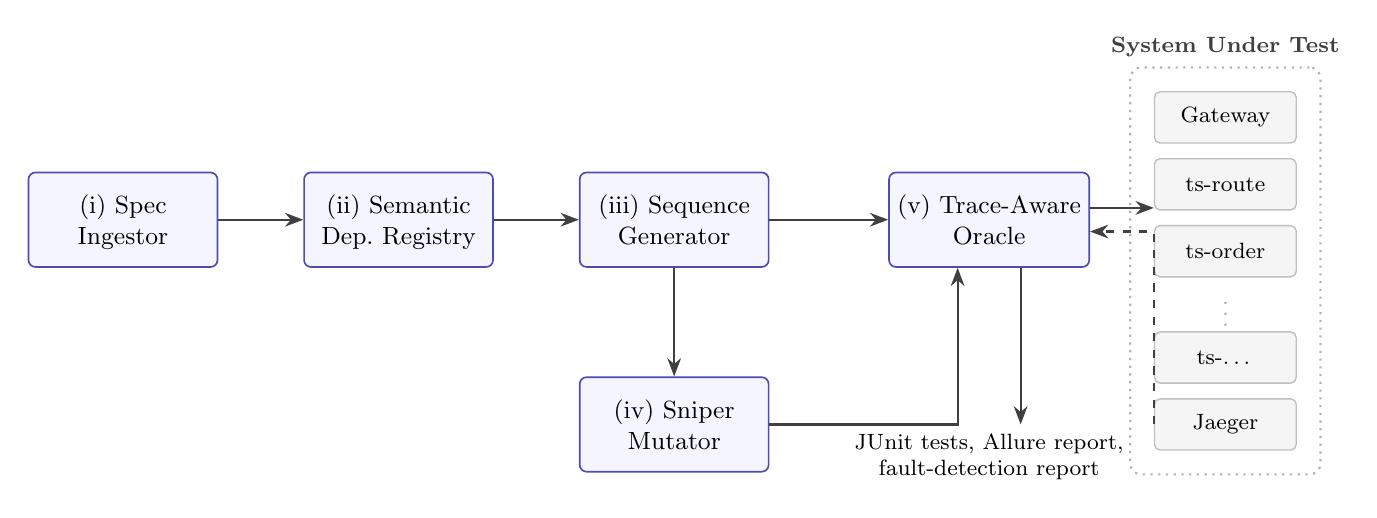
\begin{tikzpicture}[
    font=\small,
    >={Stealth[length=2.4mm]},
    comp/.style    ={draw=blue!40!gray, line width=0.6pt, rounded corners=2.5pt,
                     fill=blue!4, minimum height=12mm, minimum width=24mm,
                     align=center, inner sep=3pt, text depth=0pt},
    sut/.style     ={draw=gray!50, line width=0.5pt, rounded corners=2pt,
                     fill=gray!8, minimum height=6.5mm, minimum width=18mm,
                     align=center, inner sep=2pt, font=\footnotesize},
    sutgap/.style  ={align=center, inner sep=1pt, font=\footnotesize\itshape,
                     text=gray!70},
    outlbl/.style  ={font=\footnotesize, align=center, anchor=north},
    flow/.style    ={->, thick, >=Stealth, draw=black!75},
    backflow/.style={->, thick, dashed, >=Stealth, draw=black!75}
]

% --- Four components on the main row at y=0. ---
\node[comp] (ingest)   at ( 0.0, 0)   {(i) Spec\\Ingestor};
\node[comp] (registry) at ( 3.5, 0)   {(ii) Semantic\\Dep.\ Registry};
\node[comp] (gen)      at ( 7.0, 0)   {(iii) Sequence\\Generator};
\node[comp] (oracle)   at (11.0, 0)   {(v) Trace-Aware\\Oracle};
\node[comp] (mut)      at ( 7.0,-2.6) {(iv) Sniper\\Mutator};

% --- System Under Test cluster.  Explicit 'ts-...' row between named
%     services so the figure tells the reader 'these two are
%     representative of many'. ---
\node[sut]   (gw)   at (14.0, 1.30)  {Gateway};
\node[sut]   (svc1) at (14.0, 0.45)  {ts-route};
\node[sut]   (svc2) at (14.0,-0.40)  {ts-order};
\node[sutgap](dots) at (14.0,-1.10)  {$\vdots$};
\node[sut]   (svcn) at (14.0,-1.75)  {ts-\dots};
\node[sut]   (jgr)  at (14.0,-2.60)  {Jaeger};

\begin{scope}[on background layer]
  \node[draw=gray!60, dotted, thick, rounded corners=4pt, inner sep=3mm,
        fit=(gw)(jgr),
        label={[font=\footnotesize\bfseries, gray!50!black]above:System Under Test}] {};
\end{scope}

% --- Run output below the oracle, offset right of the mut->oracle wire. ---
\node[outlbl] (out) at (11.0,-2.6)
  {JUnit tests, Allure report,\\fault-detection report};

% --- Main horizontal pipeline. ---
\draw[flow] (ingest)   -- (registry);
\draw[flow] (registry) -- (gen);
\draw[flow] (gen)      -- (oracle);

% --- Generator -> Sniper Mutator (clean vertical). ---
\draw[flow] (gen.south) -- (mut.north);

% --- Sniper Mutator -> Oracle. ---
\draw[flow] (mut.east) -| ([xshift=-4mm]oracle.south);

% --- Oracle <-> SUT.  Two parallel arrows distinguished by +/- 1.5mm y-shift. ---
\draw[flow]     ([yshift= 1.5mm]oracle.east)
            -- ([yshift= 1.5mm]oracle.east -| gw.west);
\draw[backflow] (jgr.west)
            -- ([yshift=-1.5mm]oracle.east -| jgr.west)
            -- ([yshift=-1.5mm]oracle.east);

% --- Oracle -> output (drops straight down, offset right of mut->oracle). ---
\draw[flow] ([xshift=4mm]oracle.south) -- ([xshift=4mm]oracle.south |- out.north);

\end{tikzpicture}
}
  \caption{MIST architecture and Maven module layout. \texttt{mist-core} owns all five architectural stages (spec ingest, semantic dependency registry, sequence generator, sniper strategy, trace shape oracle) and depends on no third-party source. \texttt{mist-cli} ships the launcher \texttt{mist.jar}, the JUnit/REST-Assured writer, and the test executor. \texttt{mist-llm} is LLM dispatch and call cache. Solid arrows are MIST-issued HTTP requests; the dashed arrow is the Jaeger trace pulled back per step by the Trace Shape Oracle.}
  \label{fig:arch}
\end{figure*}

MIST is a Maven reactor of three modules (Figure~\ref{fig:arch}). \texttt{mist-core} owns all five architectural stages described below and contains no third-party source code: the OpenAPI parser wrapper (\texttt{io.mist.core.spec.*}), the semantic dependency registry (\texttt{io.mist.core.registry.*}), the sequence generator (\texttt{io.mist.core.generation.MistGenerator}), the sniper fault registry (\texttt{io.mist.core.fault.*}), and the trace shape oracle (\texttt{io.mist.core.oracle.shape.*}) all live here. \texttt{mist-cli} ships the launcher \texttt{mist.jar}, the JUnit/REST-Assured writer, the test executor, and the SPI provider classes that let \texttt{mist-core} stay framework-agnostic. \texttt{mist-llm} is LLM dispatch and call cache. The build depends on REST-Assured, swagger-parser, Allure, and JUnit as ordinary Maven library artifacts --- every black-box REST tester does~\cite{MartinLopez2021RESTest,Arcuri2019EvoMasterTOSEM,Atlidakis2019RESTler} --- but the MIST repository does not vendor any forked third-party source.

\textbf{(i) Spec Ingestor} parses one OpenAPI spec (or aggregates per-service \texttt{/v3/api-docs}) and emits an MST configuration. The bundled TrainTicket spec carries 265 operations across 37 REST-exposed services.

\textbf{(ii) Semantic Dependency Registry} indexes producer/consumer pairs over spec and trace corpus. For every \texttt{Id}/\texttt{ID}/\texttt{uuid}-stemmed parameter, a 5-pass build mines the API and JSON path that historically produces a matching value.

\textbf{(iii) Sequence Generator (Root API Mode)} runs a 5-phase pipeline (Phase 2.5 dedup, shared-pool, Phase 3 weakly-connected-component shattering, Phase 3.5 dedup, Phase 4 decomposition). On the 27 bundled traces the pipeline produces 15--20 multi-root sequences. Root API Mode (\S\ref{sec:rootmode}) keeps gateway-entry calls and prunes internal spans; the writer emits one JUnit step per root call.

\textbf{(iv) Sniper Strategy} (\S\ref{sec:sniper}) builds an \texttt{Invalid\-Input\-Pool} per parameter, keyed by \texttt{PoolKey(name, location)} so same-named params at path/query/header/cookie/body are disjoint. The 8 default categories (TYPE\_MISMATCH, REGEX\_\allowbreak MISMATCH, SEMANTIC\_MISMATCH, OVERFLOW, EMPTY, NULL, SPECIAL\_CHARACTERS, BOUNDARY\_VIOLATION) are filtered through a YAML applicability matrix and extended at run-time by \texttt{FaultMiner}.

\textbf{(v) Trace Shape Oracle} (\S\ref{sec:traceoracle}) fetches the Jaeger trace after each emitted JUnit step and evaluates three invariant families learned from a seed corpus of known-good runs. \textsc{ResponseEnvelope} subsumes the legacy \texttt{SoftErrorRuleCache}.

% =============================================================================
\section{Core Innovations}\label{sec:innov}

\subsection{Root API Mode}\label{sec:rootmode}

Internal microservice endpoints presuppose state that only specific upstream calls can mint (an \texttt{orderId} the database knows, a session token not yet expired). A generator that drives those endpoints directly must fabricate the state, and a fabrication failure is indistinguishable from a real defect (G2). Root API Mode keeps only gateway-entry HTTP spans of each Jaeger scenario --- those with no HTTP parent --- and replays them externally; internal behaviour is observed through the captured trace. The mode is one boolean (\texttt{mst.gener\-ate.only.first.step}, default \texttt{true}). Trace-grounded generation is the angle AutoRestTest~\cite{Stennett2025AutoRestTest} cannot adopt (its SPDG is derived from OpenAPI names via GloVe embedding) and that MACROHIVE~\cite{Giamattei2022MACROHIVE} adopts only at the cost of deploying a service-mesh proxy per microservice; MIST consumes whatever OTel exporter the SUT already runs.

\subsection{Sniper Strategy}\label{sec:sniper}

A negative test that mutates several parameters at once leaves the oracle unable to blame a downstream anomaly on any specific cause; a single-fault test on a non-root call has the dual problem because the trace prefix itself is driven by other, possibly mutated, values. The Sniper Strategy (Alg.~\ref{alg:sniper}) tightens both axes: one parameter, one fault category, at the first root call.

\begin{algorithm}[t]
\caption{Sniper variant generation.}\label{alg:sniper}
\begin{algorithmic}[1]
\State $r \gets$ first root call in the scenario
\State $k \gets$ round-robin pick of \texttt{PoolKey(name, location)} on $r$;\ \  $c \gets$ fault category applicable to $k$'s schema
\State $v \gets pools[r][k][c].\textrm{nextRoundRobin}()$
\State lock $(r, k, c, v)$ on the variant; fill the rest from positive sources (shared pool, smart fetch, JIT bind)
\State record $(r, k, c, v)$ as the fault target
\end{algorithmic}
\end{algorithm}

\texttt{PoolKey(name, location)} is what lets same-named parameters at path/query/header/cookie/body enrol independently. A schema-aware applicability filter rejects nonsense (no 5000-char OVERFLOW on a boolean). \texttt{FaultMiner} extends the 8-category baseline with SUT-specific entries: when the OpenAPI description cites a numeric range or regex, or when a 4xx response cites a domain-specific rejection, the miner consults the LLM, validates the proposed category against the matrix, and persists it to \texttt{mist-mined-fault-types.yaml}. The recorded $(r, k, c, v)$ tuple is what the report needs to attribute each failure to its mutation.

\subsection{Trace Shape Oracle}\label{sec:traceoracle}

\begin{figure*}[t]
  \centering
  \resizebox{\textwidth}{!}{% Figure 2: Real captured Jaeger trace from a Sniper negative variant
% against POST /api/v1/adminrouteservice/adminroute on TrainTicket.
% Trace ID: d4c577d47bcba04a00ef9b3edcbcacf6 (test_negative_POST_1_81).
% Source: src/main/resources/My-Example/trainticket/allure-results/
%         4a67e7c8-4fd2-4b6a-a698-1b1cec487a6d-attachment.txt
%
% Layout: 5-span parent-child cascade on the top, Trace-Aware Oracle
% verdict in prose underneath.  Designed to fit acmart sigconf full
% width (figure*) with the 'review' line-number gutters subtracted
% from the usable canvas.
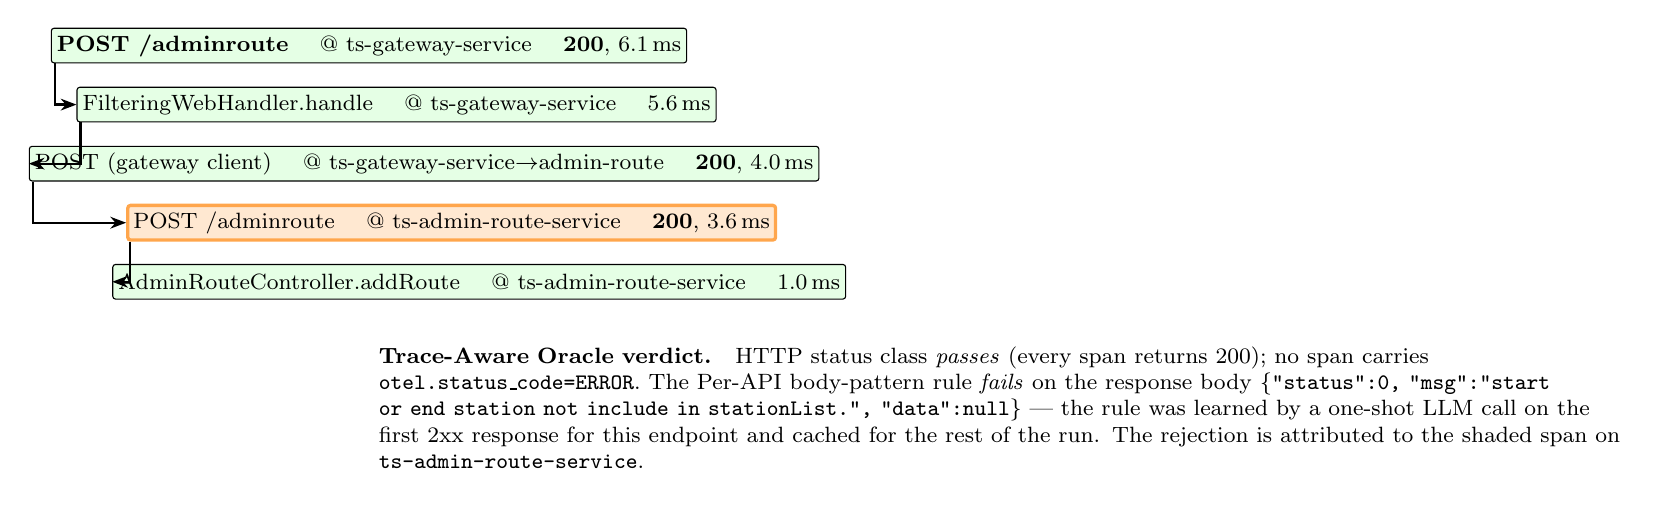
\begin{tikzpicture}[
    font=\footnotesize,
    >={Stealth[length=2mm]},
    span/.style={draw, rounded corners=1pt, minimum height=4.4mm,
                 align=left, inner sep=2pt, font=\footnotesize},
    spanok/.style={span, fill=green!10},
    spansoft/.style={span, fill=orange!18, draw=orange!70, very thick},
    edge/.style={->, thick}
]

% --- Spans: indented cascade, parent -> child ---
\node[spanok]  (s1) at (0.00, 0)
  {\textbf{POST /adminroute} \quad @ ts-gateway-service \quad \textbf{200}, 6.1\,ms};
\node[spanok]  (s2) at (0.35,-0.75)
  {FilteringWebHandler.handle \quad @ ts-gateway-service \quad 5.6\,ms};
\node[spanok]  (s3) at (0.70,-1.50)
  {POST (gateway client) \quad @ ts-gateway-service$\to$admin-route \quad \textbf{200}, 4.0\,ms};
\node[spansoft](s4) at (1.05,-2.25)
  {POST /adminroute \quad @ ts-admin-route-service \quad \textbf{200}, 3.6\,ms};
\node[spanok]  (s5) at (1.40,-3.00)
  {AdminRouteController.addRoute \quad @ ts-admin-route-service \quad 1.0\,ms};

% Parent-child arrows
\draw[edge] (s1.south west) ++(0.05,0) |- (s2.west);
\draw[edge] (s2.south west) ++(0.05,0) |- (s3.west);
\draw[edge] (s3.south west) ++(0.05,0) |- (s4.west);
\draw[edge] (s4.south west) ++(0.05,0) |- (s5.west);

% --- Trace-Aware Oracle verdict, in prose, below the trace ---
\node[align=left, anchor=north west, font=\footnotesize, text width=16cm]
  at (0,-3.7) {%
    \textbf{Trace-Aware Oracle verdict.}\quad
    HTTP status class \emph{passes} (every span returns 200);
    no span carries \texttt{otel.status\_code=ERROR}.
    The Per-API body-pattern rule \emph{fails} on the response body
    \texttt{\{"status":0, "msg":"start or end station not include in stationList.", "data":null\}}
    --- the rule was learned by a one-shot LLM call on the first 2xx response for this endpoint
    and cached for the rest of the run.
    The rejection is attributed to the shaded span on \texttt{ts-admin-route-service}.%
  };

\end{tikzpicture}
}
  \caption{Captured Jaeger trace from a Sniper negative variant against \texttt{POST /api/v1/adminrouteservice/adminroute} (trace \texttt{d4c577d4\dots\,acf6}). Every span returns HTTP 200 and no \texttt{otel.status\_code=ERROR} is set; the \textsc{ResponseEnvelope} invariant catches the soft error and the trace pins it to \texttt{ts-admin-route-service}.}
  \label{fig:trace}
\end{figure*}

The Trace Shape Oracle reaches the right verdict on Figure~\ref{fig:trace} by combining three learned-then-checked invariant families:
\begin{itemize}\setlength{\itemsep}{1pt}
  \item \textsc{SpanTreeShape}: the trace tree matches the structural pattern recorded for the same root API; a missing internal hop surfaces even when every observed call returns 200.
  \item \textsc{StatusPropagation}: no descendant span carries \texttt{otel.\allowbreak status\_code=ERROR} or \texttt{http.status\_code}~$\geq 400$.
  \item \textsc{ResponseEnvelope}: body-pattern rules (success/failure sets, field-level checks) learned per API via a one-shot LLM call on the first 2xx response and cached at \texttt{.mist/trace-shape-invariants.json}. This is the invariant on which the \texttt{status:0, data:null} envelope of the motivating example fails; it subsumes the legacy \texttt{SoftErrorRuleCache}.
\end{itemize}
We deliberately exclude timing-based invariants: in microservice deployments, end-to-end latency is dominated by cold-cache, GC, and cluster-load variance that falls within the scope of dedicated trace anomaly detection rather than functional testing. The three retained invariants operate on trace metadata that survives the PII-stripping common to GDPR/HIPAA-compliant OTel exporters --- span tree, HTTP status codes, and one-shot LLM body classification --- so MIST remains effective on production-realistic trace corpora where request/response bodies have been redacted upstream. Caching makes the LLM cost bounded: roughly two calls per distinct API regardless of how many tests touch it. The oracle also matches the response \texttt{faultName} against the injected-fault registry to attribute confirmed failures to their $(r, k, c, v)$ mutation.

% =============================================================================
\section{Usage and Case Study}\label{sec:case}

Three steps from a fresh clone:
\begin{lstlisting}[basicstyle=\scriptsize\ttfamily,frame=none]
$ mvn -DskipTests install
$ export DEEPSEEK_API_KEY=...     # or use Ollama
$ java -jar mist-cli/target/mist.jar \
    .../My-Example/trainticket-demo.properties
\end{lstlisting}
The bundled \texttt{.properties} points at the public TrainTicket deployment, the 265-operation OpenAPI spec, and 27 captured traces; an Allure report and fault-detection summary land in \texttt{target/}. The default LLM backend is DeepSeek over an OpenAI-compatible HTTP shim; a local Ollama backend with Qwen3-Coder-30B is verified end-to-end and is the configuration the numbers below are reported on. Table~\ref{tab:faults} reports detection on the bundled TrainTicket 10-fault corpus against RESTest~\cite{MartinLopez2021RESTest} and EvoMaster~\cite{Arcuri2019EvoMasterTOSEM} at a matched 25\,h budget. MIST detects 10/10; \textsc{ResponseEnvelope} is the decisive signal for soft-error cases (e.g.\ \textsc{Invalid\_Station\_Name}) where status-class alone would record a pass.

\begin{table}[t]
\centering
\caption{Detection on the bundled TrainTicket 10-fault corpus (25\,h budget each).}
\label{tab:faults}
\footnotesize
\begin{tabular}{@{}lccc@{}}
\toprule
\textbf{Fault} & \textbf{MIST} & \textbf{RESTest~\cite{MartinLopez2021RESTest}} & \textbf{EvoMaster~\cite{Arcuri2019EvoMasterTOSEM}} \\
\midrule
\textsc{Insufficient\_Stations}        & \checkmark & \checkmark & \checkmark \\
\textsc{Invalid\_Station\_Name\_Length}& \checkmark & --         & \checkmark \\
\textsc{Invalid\_Contacts\_Name}       & \checkmark & --         & \checkmark \\
\textsc{Invalid\_Seat\_Number}         & \checkmark & \checkmark & \checkmark \\
\textsc{Invalid\_Price\_Rate}          & \checkmark & --         & \checkmark \\
\textsc{Invalid\_Route\_Id}            & \checkmark & --         & --         \\
\textsc{Invalid\_Station\_Name}        & \checkmark & --         & --         \\
\textsc{Invalid\_Station\_Length}      & \checkmark & \checkmark & \checkmark \\
\textsc{Invalid\_Trip\_Id\_Format}     & \checkmark & --         & --         \\
\textsc{Invalid\_Trip\_Id\_Length}     & \checkmark & --         & --         \\
\midrule
\textbf{Total} & \textbf{10/10} & 3/10 & 6/10 \\
\bottomrule
\end{tabular}
\end{table}

% =============================================================================
\section{Related Work and Limitations}\label{sec:rw}

\textbf{Related work.} MACROHIVE~\cite{Giamattei2022MACROHIVE,Giamattei2024MACROHIVE} reaches grey-box visibility by deploying a per-service mesh proxy; MIST achieves the same observation surface vendor-neutrally via OTel. AutoRestTest~\cite{Stennett2025AutoRestTest} explores operation/parameter/value/dependency/header axes with MARL agents over a GloVe-embedded dependency graph; LogiAgent~\cite{Zhang2025LogiAgent} asks an LLM to read each response body; neither ingests traces. Distributed tracing originates with Dapper~\cite{Sigelman2010Dapper}, is standardised by OpenTelemetry~\cite{OpenTelemetry}, and trace-RCA work in production diagnostics (e.g.\ TraceRCA~\cite{Li2021TraceRCA}) uses traces as a post-hoc explanation; to our knowledge MIST is the first open-source REST tester to treat trace shape as a first-class \emph{generation} input \emph{and} oracle target.

\textbf{Limitations.} MIST requires that the SUT export OTel/Jaeger traces; uninstrumented services are invisible. The bundled case study covers one SUT (TrainTicket); a broader head-to-head against AutoRestTest, LogiAgent, and MACROHIVE across Sock Shop, Online Boutique, and DeathStarBench~\cite{Gan2019DeathStarBench} is in-progress companion work and reserved for the full research paper. This demo paper claims the tool exists, runs reproducibly from one properties file, and clears the engineering bar.

\bibliographystyle{IEEEtran}
\bibliography{refs}

\end{document}
